\chapter{基于多尺度邻域的毫米波点云配准方案}
本章的主要工作内容是优化毫米波雷达点云的迭代配准,通过分析现有配准算法在毫米波雷达点云配准上表示的不足,结合毫米波雷达点云特征,展开相应研究。本章提出了一个结合毫米波雷达多普勒特征以及点云中多尺度邻域特征的特征提取方案以及基于全局特征的配准方案。首先,结合点的多普勒特征以及点的法向量估计提升点云局部特征丰富度;其次,提出了根据多个邻域半径提取多尺度邻域特征的毫米波雷达点云特征提取网络,使用多尺度邻域的融合的方式对抗稀疏性;然后,结合源点云和参考点云特征提出了全局配准参数预测网络,使用提取的全局特征预测一次迭代中的配准参数,加快点云配准的收敛速度;最后,使用提取出的点云特征结合空间坐标进行迭代配准优化。

\section{毫米波雷达点云配准概述}
\subsection{毫米波雷达点云配准问题分析}
随着毫米波雷达点云成像技术在自动驾驶等行业中的广泛运用,毫米波雷达点云配准的准确性与鲁棒性成为研究热点。然而,由于毫米波雷达点云的分辨率低、点云稀疏、以及点云密度不均匀等特点,使得在点云稀疏区域难以有效提取特征,且在密集区域提取的特征不适用于稀疏区,传统的点云刚性配准方法难以有效配准。因此,迫切需要一种能够有效提取毫米波雷达点云特征且适应其分布特征的配准方案。
\subsection{毫米波雷达点云配准方案设计}
基于上述问题分析,本章设计了基于多尺度邻域的毫米波雷达点云配准方案。该方案主要由点级别的领域特征提取网络和全局配置参数预测网络两个部分组成。本章特别关注特征提取的优化,在点级别特征提取中,通过挖掘毫米波雷达点云的多普勒等特征,结合计算点拟合平面估计法向量,引入深度学习网络以提升点云的特征表示能力,克服了无法刚性旋转无法直接用于毫米波雷达点云的缺点,使用点于点的特征关系预测点云配准后位置,从而增强配准效果。在全局特征提取方面,通过拼接两个点云的信息,采用端到端的网络优化配置参数,以加速配准的收敛速度。相对于传统的特征提取方法,深度学习网络的引入有望在全局特征捕捉方面取得更显著的进展,从而使得配准过程更加迅速高效。基于多尺度邻域的毫米波雷达点云配准从毫米波雷达点云数据处理与增强、多尺度邻域特征提取、全局特征提取配准参数预测三个方面完成了配准。主要流程如图\ref{fig:配准流程}所示。


\begin{figure}[htbp]
	\centering
	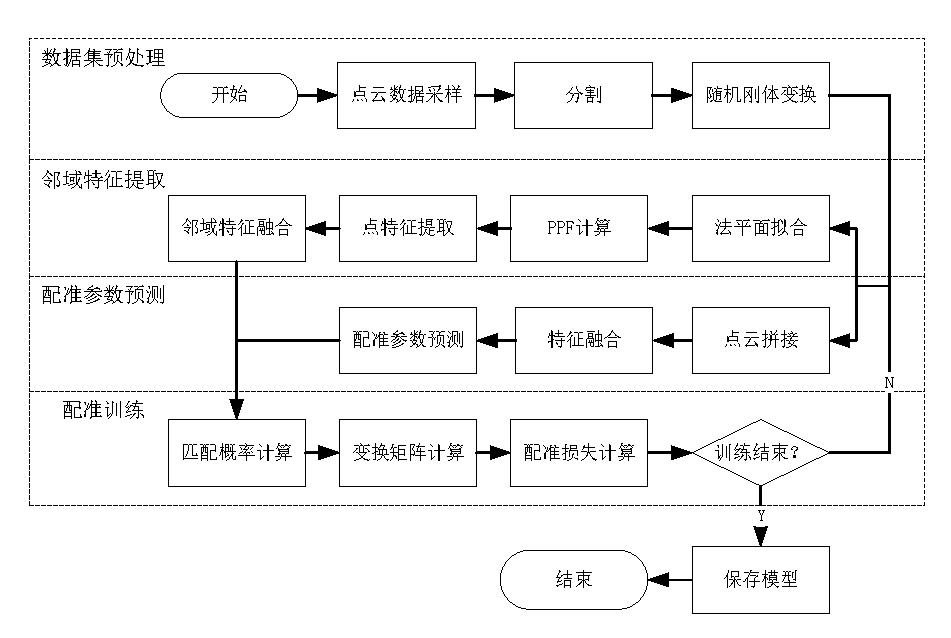
\includegraphics[width=0.9\linewidth]{figures/配准流程.pdf}
	\caption{配准流程}
	\label{fig:配准流程}
\end{figure}


\section{多毫米波雷达点云配准方案} \label{sec:配准方案整体设计}

% 在点云数据预处理阶段,使用拟合平面法向量的方式丰富点云的局部特征,在点级别特征提取中,结合多普勒特征以及法向量特征使用多尺度邻域的融合的方式对抗稀疏性,提高特征的密度。在全局特征提取阶段以及配准阶段,使用源点云与参考点云的特征拼接,使用配准参数预测网络预测一次迭代中的配准参数,计算点云亲和度,使用预测参数对源点云进行变换加快点云配准的收敛速度,得到变换后的点云,再次提取特征,直到满足迭代次数或者收敛条件。

\subsection{毫米波雷达点云数据处理与增强}
为获取有效标注的点云数据,需要对已知点云数据进行预处理。本方案使用了自采集数据集和Coloradar数据集\cite{ColoRadar}。为了使模型对不同角度、位置和噪声具有鲁棒性,需要对原始点云进行采样和变换,并且从原始点云中分离出源点云和参考点云对源点云进行旋转和平移操作,记录变换矩阵的逆矩阵用于损失的计算。
\par
(1)数据采样。为了增强模型的鲁棒性,采用多种不同的数据增强策略。第一种方式是进行均匀重采样,并打乱点云的顺序;第二种方式是引入高斯噪声,并打乱点云的顺序;第三种方式是进行随机裁剪、均匀重采样、引入高斯噪声,并打乱点云的顺序。这些采样方式的使用旨在模拟不同姿态和位置下的点云变化,提高模型的鲁棒性。
\par
(2)点云分割和随机刚体变换。点将已知点云分割为源点云和目的点云,对源点云加入包括旋转和平移的刚体变换,记录下变换矩阵用于损失的计算。首先,根据一个随机因子,确定旋转和平移的最大幅度。其次,通过生成一个随机的特殊正交群上的旋转矩阵\cite{cuisenaire1999fast},将旋转限制在三维空间内。然后,生成一个在指定范围内均匀分布的随机平移向量。生成的变换参数被组合成一个随机刚性变换矩阵,这个变换矩阵被应用到源点云上,同时确保法向量也受到旋转影响,得到一个变换后的点云。最后,计算这个变换矩阵的逆矩阵和估计矩阵,用于后续的处理,处理过程如图\ref{点云变换}所示。


将点云分割,假设原始点云为 $X$,分割后得到两个点云$P$和$Q$。对点云$P$加入包括旋转和平移的刚体变换,得到旋转矩阵 $R$ 和平移向量$T$。为了叙述简单,接下来的步骤中先忽略平移向量$T$。这一过程可以表示为:

\begin{equation}
P' = PR
\end{equation}

其中,\(P'\) 是经过刚性变换后的点云 \(P\)。
\begin{figure}[htbp]
	\centering
	% Requires \usepackage{graphicx}
	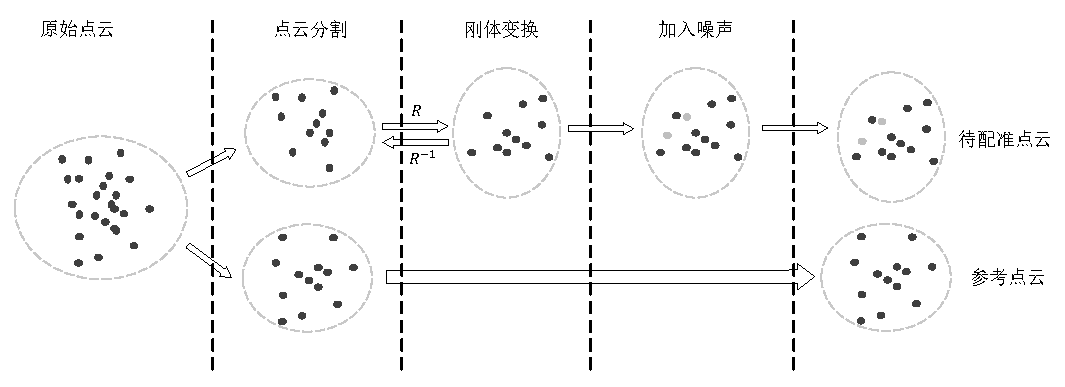
\includegraphics[width=0.96\linewidth]{figures/点云变换.pdf}\\
	\caption{点云刚体变换}
	\label{点云变换}
\end{figure}

为了得到从$P'$到$P$的变换,由公式\eqref{eq:inverse}可知,需要计算旋转矩阵 \(R\) 的逆矩阵 \(R^{-1}\),并记录。
\begin{equation}
	\label{eq:inverse}
P'R^{-1} = PRR^{-1} = P
\end{equation}

逆矩阵的计算公式如\eqref{eq:inverseMatrix}所示,其中,\(R^T\) 表示矩阵 \(R\) 的转置。最终,得到的旋转矩阵的逆矩阵 \(R^{-1}\) 可用于将经过刚性变换后的点云 \(P'\) 还原回原始位置。
\begin{equation}
	\label{eq:inverseMatrix}
R^{-1} = \frac{A^*}{\|R\|}
\end{equation}

数据集处理过程的算法描述如\ref{alg:pointcloudtransform}所示,最终得到的$R^{-1}$就是$P'$与$Q$配准的真实变换,记为$R_{gt}$。
 
\begin{algorithm}[htbp]
	\caption{点云的旋转矩阵计算}
	\label{alg:pointcloudtransform}
	\begin{algorithmic}[1]
		\Require 原始点云 $X$,
		\Ensure 旋转后点云 $P'$, 旋转矩阵的逆矩阵$R^{-1}$
		\State 在$X$中加随机的噪声
		\State 将$X$ 分割为 $P$和$Q$
		\State 在$P$应用旋转和平移矩阵: $P' = RP + T$
		\State 计算旋转矩阵的逆矩阵$R^{-1} = R^T$
		\State \textbf{return} 旋转后的点云 $P'$, 旋转矩阵的逆矩阵 $R^{-1}$
	\end{algorithmic}
\end{algorithm}

(3)法向量估计与PPF计算。点对特征(Points Pairs Features,PPF)\cite{hinterstoisser2016going}是描述两个点之间几何关系的一种表示方法。PPF的结果具有旋转不变形,因为点云配准中的源点云与目的点云之间具有旋转平移的强相关性\cite{5540108},所以PPF结果作为特征能够极大的提升配准效果。PPF的计算基于点的本地几何特性,包括它们的位置和法向量。为了提取点云所在位置的法向量,常见的方案有最小二乘拟合平面求法向量和使用深度图的法向量估计。为了计算速度以及效率的平衡,本方案使用的方法是获取领域内与目标点最近2个点,使用三个点所确定如图\ref{三点平面法向量}所示平面,用此平面法向量代替目标点的法向量。使用KD树如算法\ref{alg:kdtree}所示获取邻域内$k$个点中最近的2个点并且确保这2个点不共线。假点$p_c$设领域内最临近2个点的分别为$p_1,p_2$,从点$p_c$到这两个点的向量为:
\begin{equation}
	\begin{split}
		p_1 - p_c = (x_1 - x_c, y_1 - y_c,z_1 - z_c)\\
		p_2 - p_c = (x_2 - x_c, y_2 - y_c,z_2 - z_c)
	\end{split}
\end{equation}

\begin{figure}[htbp]
	\centering
	% Requires \usepackage{graphicx}
	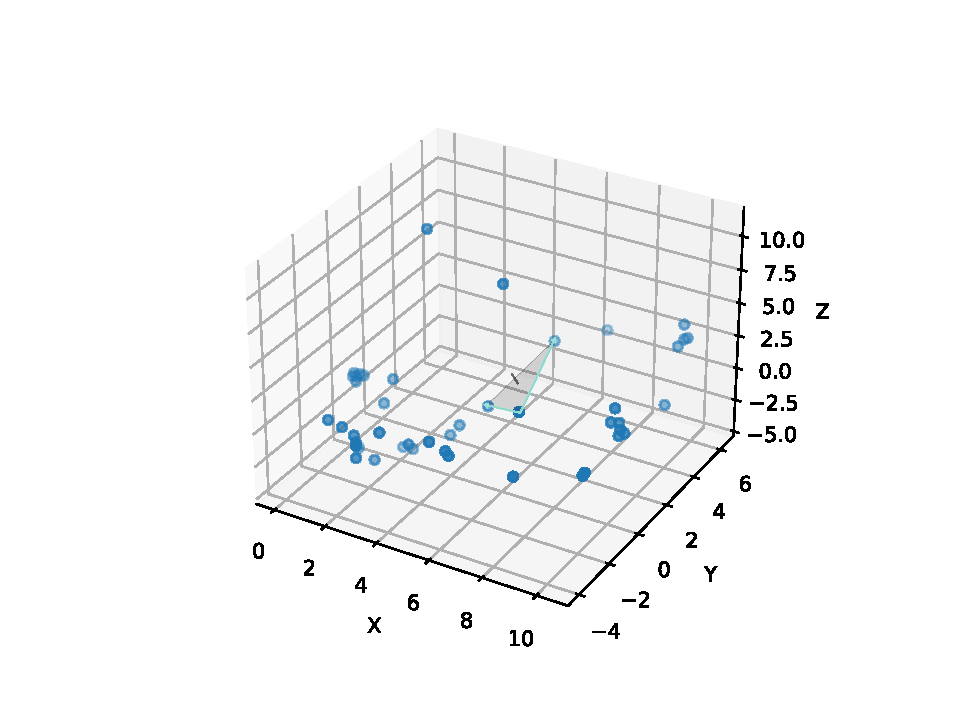
\includegraphics[width=0.7\textwidth]{figures/三点法向量.pdf}\\
	\caption{点所在平面法向量}
	\label{三点平面法向量}
\end{figure}

因为平面的法向量可以通过平面上的两个非共线向量进行叉乘(向量积)得到,拟合平面的法向量计算公式如\eqref{norm}所示,得到的向量$n$用来代替$p_c$的法向量。
\begin{equation}
	\label{norm}
	n = (p_1 - p_c) \times(p_2 - p_c) 
\end{equation}

假设$p_c,p_1$的法向量分别为$n_c,n_1$,$d = p_1-p_c$,$PPF$运算的公式如\eqref{ppf公式}所示,其中$\|d\|$是向量$d$的模长,$\angle(x, y)$是两个矢量的夹角,且$\angle(x, y) \in [0, \pi]$。

\begin{equation}
	\label{ppf公式}
		PPF(p_c,p_1) = \big(\|d\|^2,\angle(n_c, d),\angle(n_1, d),\angle(n_c, n_1) \big)
\end{equation}



\subsection{基于多尺度邻域的点特征提取}
相比于激光雷达点云,毫米波雷达的点云在精度上往往只能达到厘米级,这导致毫米波雷达的点云稀疏且不均匀,为了挖掘出毫米波雷达点云中点级别更多有意义的特征,本节受到PointNet++的启发,使用多尺度邻域特征融合的方式\cite{qi2017pointnet++},将多个邻域半径邻域的特征融合后作为点的特征表示。

多尺度邻域融合允许网络在不同尺度上获取信息,使其能够更全面、准确地理解点云的结构。采用多尺度邻域融合能够在多个尺度上对点云密度稀疏的局部区域进行特征提取\cite{RJXB202304025},提高特征密度提供更精细的匹配信息,改善点云配准的准确性。在单个邻域半径上,点邻域特征提取网络如图\ref{点特征提取网络}所示,$p_c$为待提取特征的点,假设点$x_c$周围距离不超过阈值$\tau$的邻域内有$k$个点,$p_1,p_2,\cdots,p_k$为邻域点,$\tau$由点云的密度确定。点特征提取网络的输入特征包括每个点的笛卡尔坐标$(x,y,z)$,邻域内每个点$p_i$与$p_c$的坐标差值$\Delta p_{c,i}$,点的极坐标$(\rho,\theta,\sigma)$,以及当前点的多普勒值$d$。$\Delta p_{c,i}$计算公式如\eqref{delta}所示。
\begin{equation}
	\label{delta}
	\Delta p_{c,i} = p_c - p_i
\end{equation}

除以上信息外,使用拟合平面的方式为点$x_c$估计法向量并在提取的特征信息中加入了点$x_c$与领域中每一个点的点对特征计算结果,用于表示点与局部邻域的相关性。


\begin{figure}[htbp]
	\centering
	% Requires \usepackage{graphicx}
	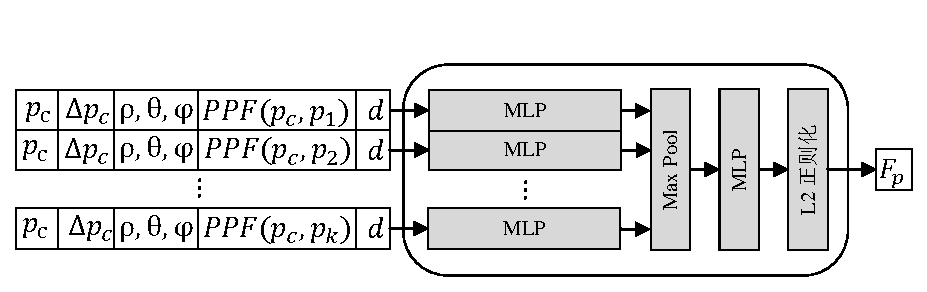
\includegraphics[width=\linewidth]{figures/点特征提取网络.pdf}\\
	\caption{点邻域特征提取网络}
	\label{点特征提取网络}
\end{figure}



假设三个邻域半径的取值为$\tau_1, \tau_2, \tau_3$,多尺度特征提取网络如图\ref{多尺度特征提取网络}所示,图\ref{多尺度特征提取网络}为图\ref{点特征提取网络}分别在三个邻域尺度之上进行迭代特征提取,对提取后的特征进行融合得到点最终的邻域特征。提取点$\tau$邻域特征的步骤如下:
\par 

(1)选取中心点$p_c$以及邻域点$p_1, p_2, \cdots, p_{k-1}$共$K$个点,输入特征为中心点坐标$(x,y,z)$,中心点多普勒$d$,中心点极坐标$(\rho, \theta, \varphi)$,以及通过公式\eqref{norm}选取领域半径。记此时特征向量的维度为$(B,N,C)$,$B$为Batch,$N$为点云中点的数量,$C$为特征通道数,此时$C$如公式\eqref{C1}所示。

\begin{equation}
	\label{C1}
	C_1 = (x,y,z,\rho,\theta,\varphi,d)
\end{equation}
\begin{figure}[htbp]
	\centering
	% Requires \usepackage{graphicx}
	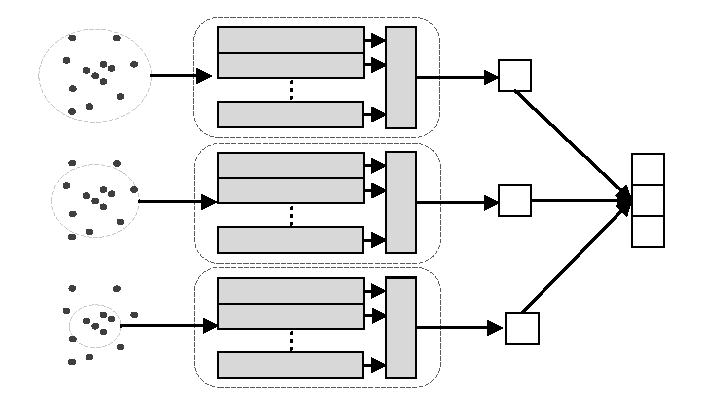
\includegraphics{figures/多尺度特征提取.pdf}\\
	\caption{多尺度特征提取网络}
	\label{多尺度特征提取网络}
\end{figure}

(2)根据邻域半径$\tau$,获取球形邻域内的点计算得到的$\Delta x$,$\Delta y$,$\Delta z$,$PPF(p_1, p_i)$,假设邻域内有$n\_samples$个点,此时得到$n\_samples\times C_2$的特征向量如\eqref{nc2}所示。
\begin{equation}
	\label{nc2}
	\begin{aligned}
		\Delta x_1, \Delta y_1, \Delta &z_1, PPF(p_c, p_1)\\
		\Delta x_2, \Delta y_2, \Delta &z_2, PPF(p_c, p_2)\\
		&\vdots \\
		\Delta x_k, \Delta y_k, \Delta &z_2, PPF(p_c, p_k)
	\end{aligned}
\end{equation}

(3)拼接特征,由于点$p_c$的特征为$1\times7$,为了保证维度的一致性,先把特征向量扩展$(B,N,1,C)$,为了与每个邻域点的特征进行拼接,在新增的第三个维度上复制$n\_samples$次,将$p_c$特征变量扩展为$(B,N,n\_samples,C_1)$,接下来在最后一个维度上拼接邻域特征,得到最终的特征向量为$(B, N, n\_samples, C_1+C_2)$,此时特征通道数为$C=C_1+C_2=14$,特征向量如\eqref{nc12}所示。
\begin{equation}
	\label{nc12}
	\begin{aligned}
	x,y,z,\rho,\theta,\varphi,d,\Delta x_1, &\Delta y_1, \Delta z_1, PPF(p_c, p_1)\\
	x,y,z,\rho,\theta,\varphi,d,\Delta x_2, &\Delta y_2, \Delta z_2, PPF(p_c, p_2)\\
	&\vdots \\
	x,y,z,\rho,\theta,\varphi,d,\Delta x_k, &\Delta y_k, \Delta z_2, PPF(p_c, p_k)
\end{aligned}
\end{equation}

(4)对输入的特征进行二维卷积和池化操作,在图像领域进行二维卷积的时候采用的常见数据格式为$(N,C,H,W)$,N为Batch大小,C为特征通道数,H表示图片的高度,W表示图片的宽度。毫米波雷达点邻域特征提取网络的输入特征为$(B,N,K,C)$,B为Batch大小,N为点云点的数量,K为邻域中点的数量,C为特征通道。在对领域点进行卷积时需要把特征通道放到第二维后进行卷积操作,维度变换后为$(B,C,K,N)$,卷积操作后在第三个维度即邻域点维度做$Max Pooling$。


(5)对多个尺度邻域提取特征进行融合,如图\ref{多尺度特征提取网络}所示。首先选取邻域半径$\tau$的取值,根据经验取邻域半径的列表为$[0.2, 0.4, 0.8]$。依次获取邻域内特征,将所有的特征在最后一个维度进行融合,得到融合后的特征。

\subsection{基于全局特征的配准参数预测}
毫米波雷达点云通常包含复杂的场景和目标,全局特征提取有助于捕捉整个点云的全局结构和一致性信息。同时由于毫米波雷达数据可能受到多路径效应、噪声等因素的影响,通过提取全局特征,可以减小噪声和局部变化等因素对配准结果的干扰提高配准结果的鲁棒性。全局特征提取可以为配准算法提供更好的初始估计。在毫米波雷达点云中,初始估计对于收敛到准确的配准结果非常重要。全局特征可以提供一个更准确的起点,有助于加速配准过程并提高最终配准的精度。全局特征的提取步骤如下:
\par
(1)数据预处理。假设输入的原始点云数据为源点云$P$,参考点云$Q$,每个点云的形状为$(B,J,4)$。B为Batch大小,J为点云大小,4为点云的笛卡尔系坐标加上每个点的多普勒速度值。
由于毫米波雷达原始数据为极坐标系,因此需要用公式\eqref{tocart}把极坐标系转为笛卡尔坐标系。
\begin{equation}
	\label{tocart}
	\begin{aligned}
		x &= \rho \cdot \sin(\theta) \cdot \cos(\varphi) \\
		y &= \rho \cdot \sin(\theta) \cdot \sin(\varphi) \\
		z &= \rho \cdot \cos(\theta)
	\end{aligned}
\end{equation}
为了区分源点云和参考点云,在源点云右侧填充全为0的列,在参考点云在右侧填充全为1的列。


(2)特征提取。全局特征提取网络如图 \ref{全局特征提取网络}所示。特征提取网络采用编码器-池化-解码器的方案。编码器通过五层卷积核为1的卷积层堆叠,将输入数据的特征通道从5维升维到1024维。接下来,使用自适应最大池化,将高维特征映射到固定的维度将最后一维变成1维,保留了最显著的特征。在解码器部分,使用多个全连接层叠加,最后的输出层为$(B,2)$,B为Batch大小,2为输出的$\alpha,\beta$值,用于全局配置参数的设置。
\begin{figure}[htbp]
	\centering
	% Requires \usepackage{graphicx}
	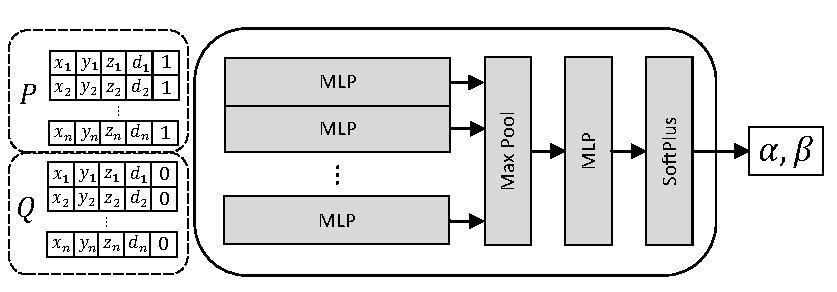
\includegraphics{figures/全局特征提取网络.pdf}\\
	\caption{全局特征提取网络}
	\label{全局特征提取网络}
\end{figure}


\subsection{训练流程}
通过上述数据预处理以及点云特征提取可以得到源点云和参考点云的特征、全局特征、源点云到参考点云的变换$R_{gt},t_{gt}$,训练流程如下:
\par
(1)计算源点云与参考点云的特征距离。使用源点云和参考点云,计算两个点云特征的欧氏距离。在经过特征提取后,源点云和参考点云的特征矩阵分别为$F_{src}$和$F_{ref}$。在三维空间两点$X,Y$之间欧氏距离的计算公式如\eqref{dist}所示。
\begin{equation}
	\label{dist}
	\begin{aligned}
		d &= (x_1-x_2)^2 +  (y_1-y_2)^2 +  (z_1-z_2)^2\\
		&= x_1^2+x_2^2 +  y_1^2+y_2^2  +  z_1^2+z_2^2 - 2x_1x_2 - 2y_1y_2 - 2z_1z_2\\
		&=x_1^2+x_2^2 +  y_1^2+y_2^2  +  z_1^2+z_2^2 - 2(x_1x_2+y_1y_2+z_1z_2)
	\end{aligned}
\end{equation}

把坐标写成向量形式分别为$X=[x_1, y_1, z_1],Y=[x_2,y_2,z_2]$,定义$sum$函数为在最后一个维度上求和,此时距离可以表示为公式\eqref{dist2}。

\begin{equation}
	\label{dist2}
	d = sum(X^2) + sum(Y^2) - 2XY^T
\end{equation}
因此,源点云和参考点云在的特征距离可以表示为公式\eqref{dist3}。

\begin{equation}
	\label{dist3}
	D_{feat} = sum(F_{src}^2) +sum( F_{ref}^2) - 2 F_{src}F_{ref}^T
\end{equation}
\par
(2)计算混合亲和度矩阵。如公式\eqref{affinity}所示,其中$ j $表示源点云中的点的索引,$k $表示参考点云中的点的索引。这个公式反映了特征之间的距离对于初始匹配矩阵值的影响。 $\beta$ 和 $\alpha$ 是预测的参数,它们用于调整特征距离对亲和力的影响。如果 $\alpha$ 是一个浮点数,那么在计算时,所有的距离都会减去相同的 $\alpha$ 值。如果$\alpha$ 是一个向量,那么每个特征点对应的距离都会减去不同的 $\alpha$ 值。$A$是一个形状与特征都和距离矩阵相同的矩阵,但其值已经根据全局参数的预测值预测的参数进行了调整。

\begin{equation}
	\label{affinity}
	A_{jk} = -\beta \cdot (D_{feat}[j,k] - \alpha)
\end{equation}
\par
(3)点匹配概率计算。为了提高数值稳定性以及加快收敛速度,对亲和度矩阵进行Sinkhorn计算\cite{cuturi2013sinkhorn}如算法\ref{alg:sinkhorn}所示,得到归一化的对数概率矩阵。当概率值趋近0或1时,使用对数运算避免了数值下溢或溢出的问题并且在数值优化中往往更容易收敛。然后将对数概率矩阵转换成概率矩阵,该矩阵表示源点与目标点之间的匹配程度。由于概率矩阵表示了每个源点与每个目标点的匹配概率,因此可以使用这些概率来计算加权目标点的坐标。每个源点的加权坐标是目标点的加权平均值,其中权重是与每个目标点相关的匹配概率。概率矩阵中的每一行和每一列都是归一化的,这意味着它们的总和都是1。这使得每个源点都有一个与之相关的匹配概率分布,其中所有概率之和为1,计算过程如算法\ref{alg:sinkhorn}所示。
\begin{algorithm}[htbp]
	\caption{Sinkhorn算法}\label{alg:sinkhorn}
	\begin{algorithmic}[1]
	\Require 对数形式的正矩阵 $log\_alpha$,迭代次数 $n\_iters$,提前终止阈值 $eps$
	\Ensure 双随机矩阵的对数 $log(perm\_matrix)$
	\State 初始化:前一迭代矩阵 $prev\_alpha \leftarrow None$
	\For{$i = 1$ to $n\_iters$}
		\State 行归一化:对每一行的 $log\_alpha$ 进行归一化,使每行元素的指数和为1
		\State 列归一化:对每一列的 $log\_alpha$ 进行归一化,使每列元素的指数和为1
		\If{$eps > 0$ \textbf{and} $prev\_alpha \neq None$}
			\State 计算当前矩阵与前一矩阵的最大绝对差值
			\If{最大差值小于 $eps$}
				\State \textbf{break}
			\EndIf
		\EndIf
		\State 更新 $prev\_alpha$ 为当前的 $log\_alpha$
	\EndFor
	\State \Return $log\_alpha$
	\end{algorithmic}
\end{algorithm}
\par
(4)计算变换。概率矩阵中的每一行和每一列都是归一化的,这意味着它们的总和都是1。这使得每个源点都有一个与之相关的匹配概率分布,其中所有概率之和为1。概率矩阵的每一行都对应于源点云中的一个点,每一列都对应于参考点云中的一个点。虽然最终目标是找出源点云的刚性变换,但是源点云与参考点云可能存在轻微的非刚性形变,通过求加权平均的方式能够缓解非刚性形变,提高配置过程的鲁棒性。将概率矩阵中的每一行与参考点云中的点进行加权求和,从而得到加权的参考点云。
使用源点云和加权参考点云计算两个点云之间的刚性变换。将两个点集分别减去对应的质心,得到质心对齐后的点集,计算质心对齐后的点集之间的协方差矩阵,对协方差矩阵进行SVD分解\cite{kalman1996singularly},得到旋转矩阵如\eqref{旋转公式}所示。根据SVD分解得到的旋转矩阵和质心,计算平移矩阵如\eqref{平移公式}所示。平移矩阵将源点云的质心转移到参考点云的质心位置。

\begin{algorithm}[htbp]
	\caption{计算刚性变换}
	\label{alg:compute_rigid_transform}
	\begin{algorithmic}[1]
		\Require 源点云 $P1$,参考点云 $P2$
		\Ensure 从 $P1$ 到 $P2$ 的旋转矩阵 $R$,平移矩阵 $t$
		\State 计算源点云的质心 $P1_c$ 和参考点云的质心 $P2_c$
		\State  $P1\_centered$ $\gets$  $P1$ -  $P1_c$, $P2\_centered$ $\gets$  $P2$ -  $P2_c$ \Comment{ 将源点云和参考点云中心化}
		\State 计算协方差矩阵 $cov = P1\_centered^\top \cdot P2\_centered $
		\State 计算两个旋转矩阵 $R_{\text{pos}}$ 和 $R_{\text{neg}}$,并选择行列式为正的矩阵
	 \State 计算平移矩阵 $translation = -R \cdot P1_c + P2_c$
		\State 将旋转矩阵和平移矩阵连接起来,得到变换矩阵 $T$
	\end{algorithmic}
\end{algorithm}
(5)设计损失函数。每个迭代步骤,将预测的变换应用到源点云上,并计算与真实变换后的源点云之间的损失。损失函数可以选择为均方误差MSE。
\begin{equation}
	loss = \frac{1}{N}\sum_{j=1}^{N}\| (RP_j+t) - (R_{pred}P_j+t_{pred}) \|^2
\end{equation}
\par
(6)迭代过程。迭代过程中,使用上述损失函数,使用Adam优化器优化学习率设置,学习率为0.0001,批大小为8,训练的epoch数量为1000,使用Early Stopping策略在模型的性能没有提升时提前结束训练。训练过程中使用学习率衰减策略,当模型的性能没有提升时减小学习率。本章模型在训练过程在验证集上各个评估指标的变化曲线如图\ref{fig:验证集评估指标变化曲线}。分析曲线可知,在前50个Epoch各个实验评估指标下降剧烈。在200到300Epoch曲线出现抖动,500Epoch后曲线的趋势开始平稳,模型逐渐收敛。
\begin{figure}[htbp]
	\centering
	\subcaptionbox{MAE(R)}{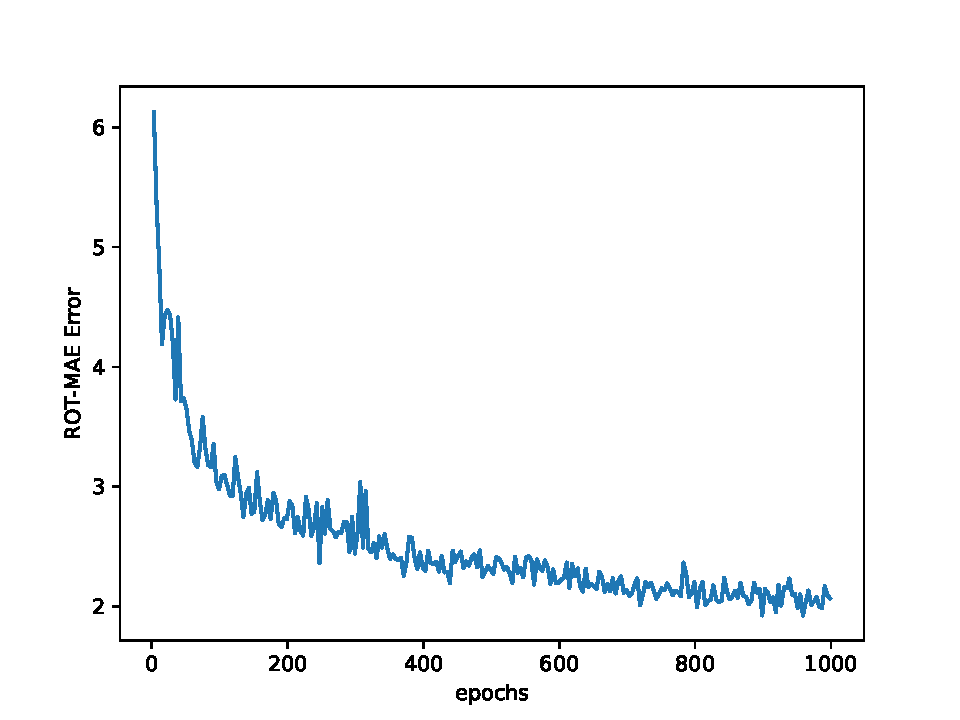
\includegraphics[width = 0.45\textwidth]{figures/rot_mae_err.pdf}}
	\subcaptionbox{RMSE(R)}{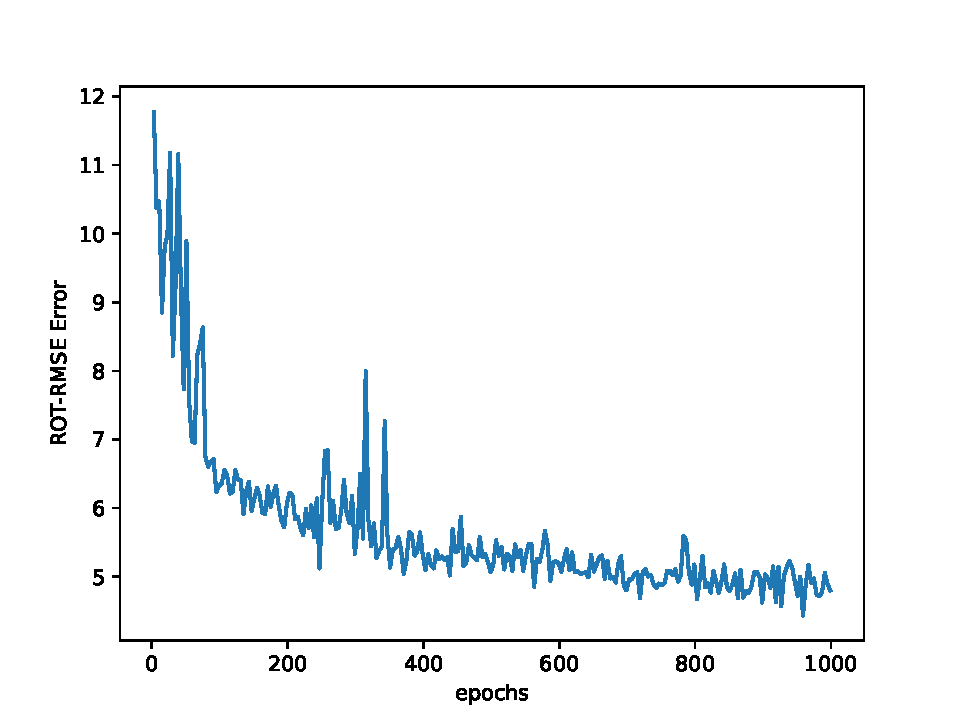
\includegraphics[width = 0.45\textwidth]{figures/rot_rmse_err.pdf}}
	\subcaptionbox{MAE(T)}{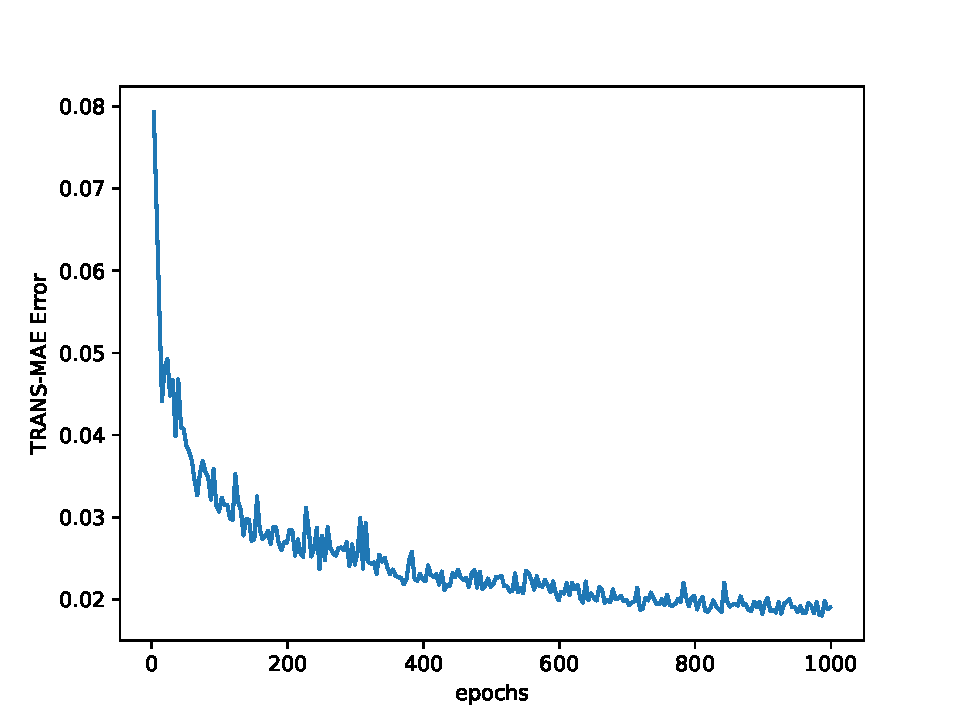
\includegraphics[width = 0.45\textwidth]{figures/trans_mae_err.pdf}}
	\subcaptionbox{RMSE(T)}{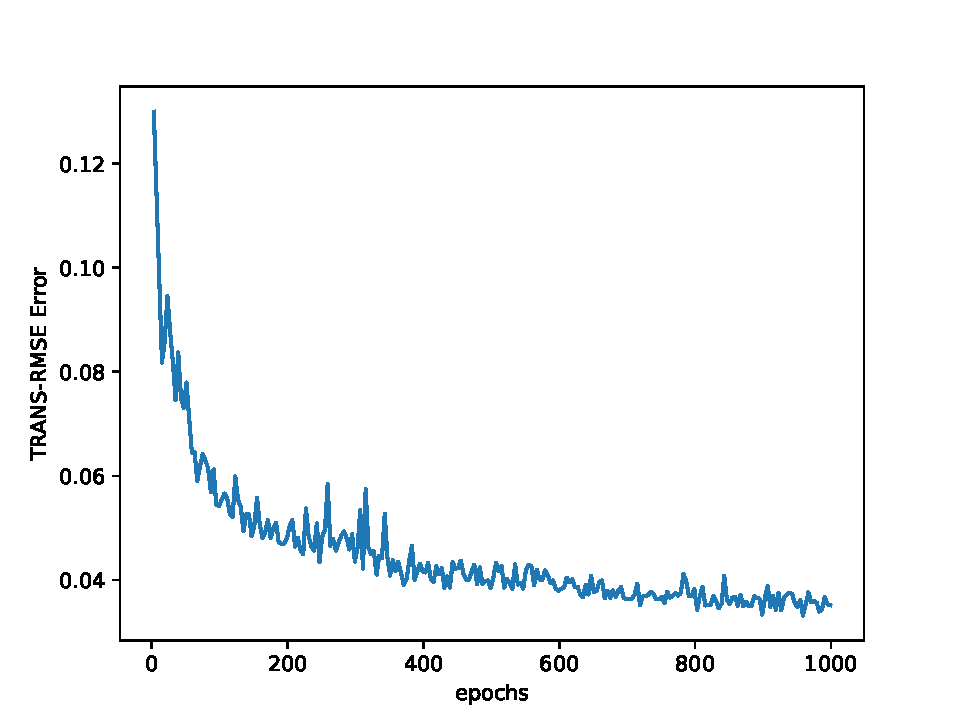
\includegraphics[width = 0.45\textwidth]{figures/trans_rmse_err.pdf}}
	% \subcaptionbox{Chamfer-Dis}{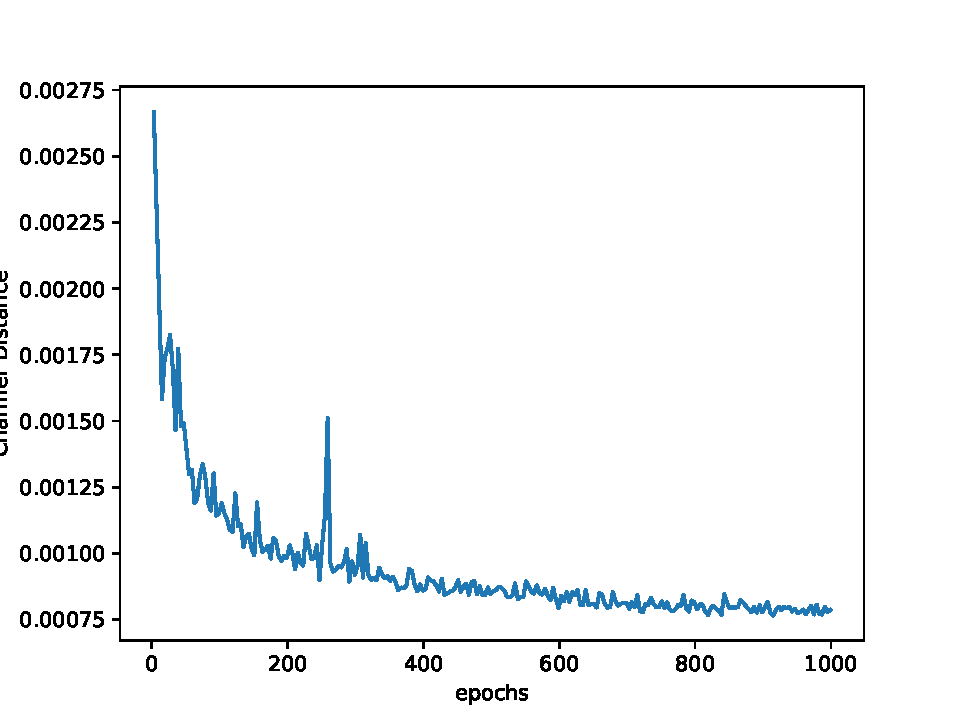
\includegraphics[width = 0.45\textwidth]{figures/cd.pdf}}
	\caption{验证集评估指标变化曲线}
	\label{fig:验证集评估指标变化曲线}
\end{figure}

\section{实验设计与结果分析}

\subsection{数据采集}
本节使用的数据集为ColoRadar数据集\cite{ColoRadar}和自采集数据集。ColoRadar数据集包含了来自街道,城市,矿山等52个序列超过145分钟的数据。ColoRadar所用毫米波雷达为AWR1843,参数设置如表\ref{第四章雷达参数表}。自采集数据集使用IWR6843采集了包含室内1到3人,室外1到3人的场景,各收集的1000组数据共计6000组数据。
两个数据集所用到的毫米波雷达参数信息如表\ref{第四章雷达参数表}所示。

\begin{table}[htbp]
	\centering
	\tabcolsep=3mm
	\caption{第四章雷达参数表}
	\begin{tabular}{ccc}
		\toprule
		参数 & IWR6843 &AWR1843 \\
		\midrule
		发射天线 & 4 &4 \\
		接收天线 &3 &3  \\
		ADC采样点数 & 128 & 96  \\
		每帧Chrip数 & 128 & 288 \\
		开始频率 &  60.6GHz &  76.9GHz   \\
		带宽 & 2.249GHz &  4GHz  \\
		空闲时间 & 10ns  & 10ns\\
		调频斜率 & 54.725MHz/us& 100MHz/us \\
		\bottomrule
	\end{tabular}
	\label{第四章雷达参数表}
\end{table}

\subsection{实验评估指标}
在刚性变换的评估指标中,平均绝对误差(MAE)、均方误差(MSE)和均方根误差(RMSE)是最常用的评价指标。本节在旋转和平移两个方面使用公式\eqref{MAE}计算平均绝对误差(MAE)使用公式\eqref{RMSE}计算均方根误差(RMSE),得到旋转均方根误差RMSE(R)、旋转平均绝对误差MAE(R)、平移均方根误差RMSE(T)和平移平均绝对误差MAE(T)作为评估指标。除此之外,使用倒角距离(Chamfer-Distance)作为评估指标。倒角距离是一种用于评估两个点云之间的距离的指标,它是两个点云之间的最小距离的平均值。两个点云$X$和$Y$之间的
倒角距离的公式表示为公式\eqref{Chamfer-Distance}所示。倒角距离越小,说明两个点云之间的距离越小,配准效果越好。
\begin{equation}
	\label{Chamfer-Distance}
	\text{Chamfer-Dis}(X,Y) = \frac{1}{|X|} \sum_{x \in X} \min_{y \in Y} \|x - y \|^2 + \frac{1}{|Y|} \sum_{y \in Y} \min_{x \in X} \|x - y \|^2 
\end{equation}
\subsection{消融实验}
为了验证本章加入多普勒特征,拟合法向量,以及多邻域特征提取的有效性,本节设置了对于特征提取部分和多尺度邻域特征提取部分进行了消融实验,通过不同的特征提取方式的组合,对比最终配准效果的各项评估指标,验证本配准方案的有效性。消融实验包含的组合方案有:
\par
(1)网络结构保持不变,在提取特征中去掉法向量。
\par
(2)在提取点邻域特征提取时,只提取固定$\tau$邻域的特征。
\par
(3)网络结构保持不变,在提取特征中去掉多普勒。
\par
(4)本方案,保留了所有的模块。
\par
各模块的组合方式和最终配准结果如表\ref{消融实验}所示。
\
\begin{table}[htbp]
	\centering
	\caption{消融实验}
	\scalebox{0.92}{
		\begin{tabular}{cccccccc}
			\toprule
			多普勒 & 法向量评估 & 多尺度邻域特征&MAE(R) & RMSE(R)& MAE(T) & RMSE(T)& Chamfer-Dis \\
			\midrule
			\Checkmark &  &  \Checkmark& 7.502 & 8.288 & 0.342 & 0.360 & 0.251 \\
			\Checkmark & \Checkmark & & 19.086 & 27.047 & 0.168 & 0.252 &  1.151 \\
			 & \Checkmark & \Checkmark& 7.469 & 21.075 & 0.361 & 0.380 & 0.429 \\
			\Checkmark & \Checkmark & \Checkmark&  6.459 & 6.904 & 0.063 & 0.166 & 0.243 \\
			\bottomrule
		\end{tabular}
	}
	\label{消融实验}
\end{table}
\par
从表\ref{消融实验}可知,添加了多普勒,法向量评估和多尺度邻域特征的配准效果最佳,当保留多普勒和法向量估计去掉多尺度邻域特征后配准效果最差,验证了多尺度邻域特征在配准过程中是至关重要的;当模型去掉多普勒或者去掉法向量评估后,配准精度损失都有了一定的上升,证明了多普勒和法向量评估的必要性;去掉多普勒后平移损失有明显的上升,证明了多普勒信息能够在点云配准中平移变量评估中起到重要作用;去掉法向量评估后平移损失和旋转损失都有明显的上升,证明了法向量评估在旋转矩阵和平移向量的评估上都有贡献。

\subsection{对比实验}
为了验证本章方案的有效性和实验评估的准确性,本节进行了三组对比实验,分别为同类型雷达点云配准实验,不同类型雷达点云配准实验,配准效率对比实验。在这三组实验中本章方法将与 ICP、Go-ICP、 RPM、FGR、 DCP、 PointNetLK、 RPMNet 进行对比。

\par
(1)同类型雷达点云配准实验。为了验证在同类型毫米波雷达点云上训练出的模型配准效果,本节在同一雷达的雷达点云数据集上训练PointNetLK模型,RPMNet模型和本章模型。
\begin{table}[htbp]
	\centering
	\tabcolsep=3mm
	\caption{同类型雷达点云配准实验结果}
	\begin{tabular}{cccccc}
		\toprule
		算法 &  RMSE(R)&MAE(R)& RMSE(T)&MAE(T) & Chamfer-Dis \\
		\midrule
		ICP&24.869&10.003&0.344&0.298&1.088\\
		GoICP&15.905&3.753&0.546&0.176&0.353\\
		RPM&6.907&1.591&0.467&0.183&0.255\\
		FGR&6.729&1.152&0.277&0.274&0.319\\
		PointNetLK&19.416&8.825&0.983&0.524&1.040\\
		DCP&7.435&3.553&0.503&0.344&0.696\\
		RPMNet&6.603&1.312&0.318&0.166&0.243\\
		本方案&6.459&1.204&0.263&0.126&0.180\\
		\bottomrule
	\end{tabular}
	\label{同类型雷达点云配准实验结果}
\end{table}

从表\ref{同类型雷达点云配准实验结果}可以看出,本方案明显优于其余7种算法。与表现最好的RPMNet相比 RMSE(R)降低了2.2\%、MAE(R)降低了8.9\%、 RMSE(T)降低了20.9\%、MAE(T)下降了35\%,证明了使用特征距离代替空间距离对于配准具有明显的提升效果。

(2)不同类型雷达点云配准实验。为了验证在不同毫米波雷达点云上训练出的模型泛化效果,本节在将在AWR1843点云数据集上训练PointNetLK模型,RPMNet模型和本章模型,并且将模型在IWR6843上进行配准使用。初始学习率为0.0001,权值衰减为0.01。


从表\ref{不同类型雷达点云配准实验结果}可以看出,传统算法在不同类型的雷达点云上配准误差没有受到太多的影响,而基于深度学习的算法PonitNetLK和DCP误差率有所上升,PonitNetLK的RMSE(R)、MAE(R)、RMSE(T)、MAE(T)、Chamfer-Dis分别上升了11.3\%、30.3\%、13\%、18.7\%、12.3\%,本方案的RMSE(R)、MAE(R)、RMSE(T)、MAE(T)、Chamfer-Dis分别上升了1.4\%、1.9\%、1.5\%、3.6\%、2.1\%,与其他基于神经网络的模型相比表现更加稳定。推测原因为神经网络在学习特征时在不同类型的点云时,由于毫米波雷达精度、采样频率等参数的不同,导致对于相同物体不同毫米波雷达点云特征有所不同。本方案使用的多尺度邻域特征提取方案能用有效克服优于采样精度和点云放缩带来的特征变化,因此能够维持配准误差的稳定性。

\begin{table}[htbp]
	\centering
	\tabcolsep=3mm
	\caption{不同类型雷达点云配准实验结果}
	\begin{tabular}{cccccc}
		\toprule
		算法 &  RMSE(R)&MAE(R)& RMSE(T)&MAE(T) & Chamfer-Dis \\
		\midrule
		ICP&20.370&10.175&0.097&0.051&1.010\\
		GoICP&16.040&4.037&0.052&0.180&0.353\\
		RPM&8.098&2.081&0.064&0.163&0.325\\
		FGR&7.552&1.465&0.044&0.214&0.184\\
		PointNetLK&21.620&11.499&0.108&0.622&0.168\\
		DCP&7.982&5.160&0.072&0.048&0.954\\
		RPMNet&7.371&2.195&0.521&0.728&0.784\\
		本方案&6.588&0.922&0.064&0.169&0.248\\
		\bottomrule
	\end{tabular}
	\label{不同类型雷达点云配准实验结果}
\end{table}

\par
(3)效率对比实验。为了比较不同的方案在同一点云上的配准速度,本节将计算多个方案分别在AWR1843和IWR6843一帧点云上的配准时间做对比,对比结果如表所示:
\begin{table}[htbp]
	\centering
	\tabcolsep=3mm
	\caption{配准效率对比}
	\scalebox{0.98}{
		\begin{tabular}{ccccccccc}
			\toprule
			点云类型 & ICP & Go-ICP& RPM & FGR & PointNetLK & DCP & RPMNet&本方案 \\
			\midrule
			IWR6843 & 0.032 & 1.85 & 0.047 & 0.043 & 0.062 &0.231 & 0.027 & \textbf{0.022} \\
			AWR1843 & 0.039 & 1.98 & 0.037 & 0.061 & 0.076 &0.331 & 0.042 & \textbf{0.029} \\
			\bottomrule
		\end{tabular}
	}
	\label{配准效率对比实验结果}
\end{table}

\section{本章小结}

本章提出了一种结合毫米波雷达多普勒特征以及点云多尺度邻域特征的特征优化毫米波雷达点云配准方案。在点云数据预处理阶段,通过为毫米波雷达点云数据拟合法平面的方式丰富点级别的空间特征信息;在特征提取阶段,为对抗点云的形变带来的特征变化引入了多普勒信息和多尺度邻域特征提取提高了配准模型的泛化能力和稳定性;在迭代阶段,使用全局特征进行参数预测加快配准的收敛。通过实验分析验证了本方案在多个信噪比、不同目标数量、不同雷达类型的点云上具有优秀的配准效果和泛化能力。